% Created 2024-10-16 śro 21:35
% Intended LaTeX compiler: pdflatex
\documentclass[../../main.tex]{subfiles}

% \usepackage[a4paper, margin=3cm]{geometry}
% \usepackage{amssymb} // not working

\usepackage[T1]{fontenc}
\usepackage[utf8]{inputenc}
\usepackage{graphicx}
\usepackage{longtable}
\usepackage{wrapfig}
\usepackage{rotating}
\usepackage[normalem]{ulem}
\usepackage{amsmath}
\usepackage{capt-of}
\usepackage{hyperref}
\usepackage{siunitx}
\usepackage{float}
\usepackage[polish]{babel}

\graphicspath{{../}}
\author{Wojciech Paderewski}
\date{\today}
\title{LDO}
\hypersetup{
 pdfauthor={Wojciech Paderewski},
 pdftitle={LDO},
 pdfkeywords={},
 pdfsubject={},
 pdflang={Polish}}

\begin{document}
Wymagania jakie musi spełnić LDO to zapewnie zasilania mikrokontrolera ESP32 oraz potencjometru cyfrowego.
Zgodnie z dokumentacją ESP32 \cite{st:esp32} pobiera on maksymalnie 340mA prądu, a potencjometr cyfrowy \cite{st:potencjometr} \SI{100}{\milli\ampere},
co daje łącznie \SI{440}{\milli\ampere}. Układ LDO ma być zasilany \SI{5}{\volt}, a na wyjściu ma być \SI{3.3}{\volt}.

Wybrano układ LDO AP7363 firmy Diodes Incorporated \cite{st:ldo}, jest to układ LDO o napięciu wyjściowym \SI{3.3}{\volt} i prądzie wyjściowym \SI{1.5}{\ampere},
co daje duży zapas wydajności prądowej. Układ ten jest dostępny w obudowie TO252, co pozwala na łatwy montaż na płytce drukowanej. Producent zaleca podłączenie układu
zgodnie z rysunkiem \ref{fig:ldo_datasheet}.

\begin{figure}[H]
    \centering
    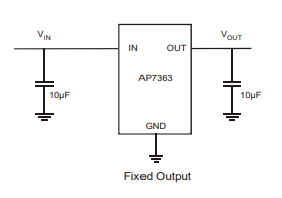
\includegraphics[width=0.5\textwidth]{ldo_datasheet.png}
    \caption{Schemat podłączenia LDO zalecany przez producenta \cite{st:ldo}}
    \label{fig:ldo_datasheet}
\end{figure}

Względem schematu zaproponowanego przez producenta, zdecydowano się na zastosowanie dodatkowo kondensator ceramiczny o pojemności \SI{100}{\nano\farad}, by zminimalizować zakłócenia.
Dodano po kondensatorze na wejście i wyjście układu równolegle do kondensatorów \SI{10}{\micro\farad} zaproponowanych przez producenta. 
Schemat elektryczny układu LDO przedstawiono na rysunku \ref{fig:ldo}.

\begin{figure}[H]
    \centering
    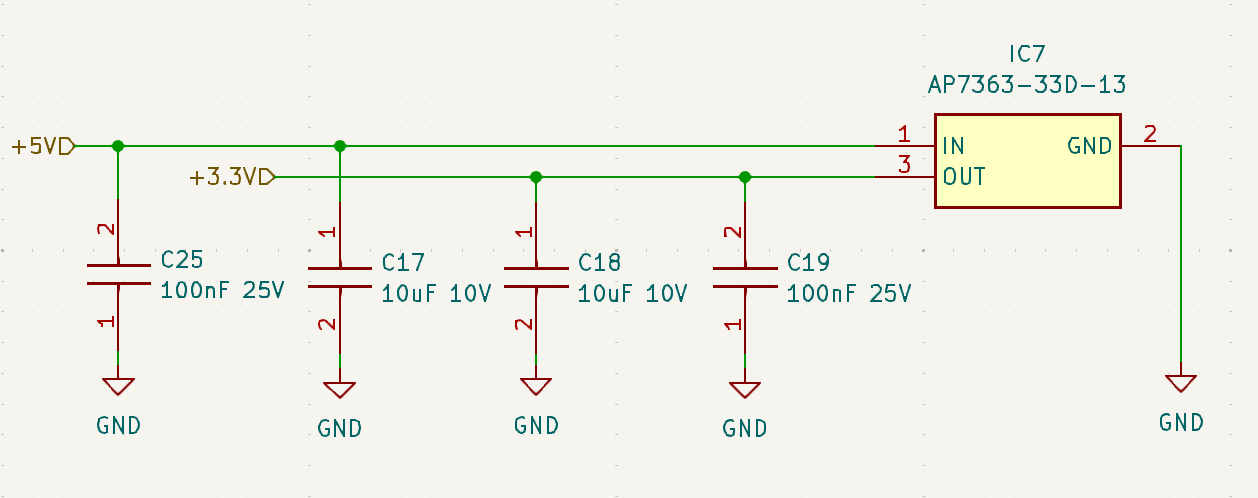
\includegraphics[width=0.8\textwidth]{LDO.png}
    \caption{Schemat elektryczny układu LDO}
    \label{fig:ldo}
\end{figure}

\end{document}
